\documentclass{article}
\usepackage[utf8]{inputenc}
\usepackage[top=1in, bottom=1in, left=1in, right=1in]{geometry}
% \usepackage{indentfirst}
\usepackage{amsmath}
\usepackage{amssymb}
\usepackage{mathtools}
\usepackage{graphicx}
    \DeclareGraphicsExtensions{.png, .jpeg}
\usepackage{caption}

% custom macros
\newcommand*{\doublebar}[1]{\overline{\overline{#1}}}
\newcommand*{\unknown}[0]{\;?\;}
\DeclareMathOperator*{\argmax}{argmax}


% main document
\title{MATH 786: Cooperative Game Theory \\ HW03}
\author{Terence Henriod}
\date{\today}

\begin{document}

\maketitle

\begin{abstract}
Convex Games, Balanced Games, Shapley-Bondareva Theorem, Market Games.
\end{abstract}


\newpage
\begin{enumerate}
\item It turns out that the glove game (from HW \#1 and HW \#2) is an assignment game. To show that you understand this, give the assignment matrix $C$ that represents a glove game with two ``left-glovers" and four ``right-glovers". \\

\textit{Solution}: \\
\\
\begin{center}
\begin{tabular}{ c | c | c | c | c |}
        & $p_{1}$ & $p_{2}$ & $p_{3}$ & $p_{4}$ \\
\hline
$m_{1}$ & 5       & 5       & 5       & 5 \\
\hline
$m_{2}$ & 5       & 5       & 5       & 5 \\
\hline 
\end{tabular}
\end{center} \hfill\\
% \[
% C = \begin{pmatrix}
%   5 & 5 & 5 & 5 \\
%   5 & 5 & 5 & 5
% \end{pmatrix}
% \]

%
\item
    \begin{enumerate}
    \item Are all assignment games convex? Give an argument or counterexample. \\

    \textit{Solution}: \\

    All assignment games are convex.

    By a similar argument as on the last home work. We know that assignment games are balanced, so any arbitrary assignment is balanced. Since the sub-games of an assignment game would also be
    assignment games, they are also arbitrary market games that are balanced. Since all of the original arbitrary assignment game's sub-games are balanced, it is totally balanced. All totally balanced games are convex games. \\

    %
    \item Are all assignment games market games? Give an argument or counterexample. \\

    \textit{Solution}: \\

    All assignment games are market games.

    In the previous homework, we found that all market games are convex games (by a similar argument in the previous question), so since assignment games are convex, they are market games also (Just get creative by having one class of good for each seller, and utility functions that only get value from having goods assigned to buyers).

    % I am wondering if matching games are not assignment games because the goods can only be transferred in discrete units (namely precisely 1 item may be transferred from a seller to a buyer), so I am not sure if that violates the requirement that utility functions must be continuous and increasing.
    %
    % Recall that a market game is defined by it's player set ($N$), the set of goods in the market ($M$), the initial endowments of those goods to players ($\{\vec{a}\}$), and the utility functions of those goods for the players ($\vec{u}$). An assignment game is simply a market game where the $\ell$ and $\m$ combine to form $N$; the set of goods has the same cardinality as $\ell$, with one element or good for each seller; the initial endowments are all allotted to each seller, and there is only $1$ of each good in the game, $1$ for each seller's product; finally, the utility functions represent the net gain for a buyer-seller pair should they be matched, utility functions for sellers do not produce value, utility functions for buyers have value.

    %
    \end{enumerate}

\item Consider the assignment game defined by the matrix
\[
C = \begin{pmatrix}
  $4$ & $x$ \\
  $x$ & $4$
\end{pmatrix}
\]
where $0 \le x \le 4$.

    \begin{enumerate}
    \item Graph the core of this game, in terms of utility payoffs for the sellers, as a function of $x$. \\

    \textit{Solution}: \\
    \begin{figure}[h!]
      \centering
      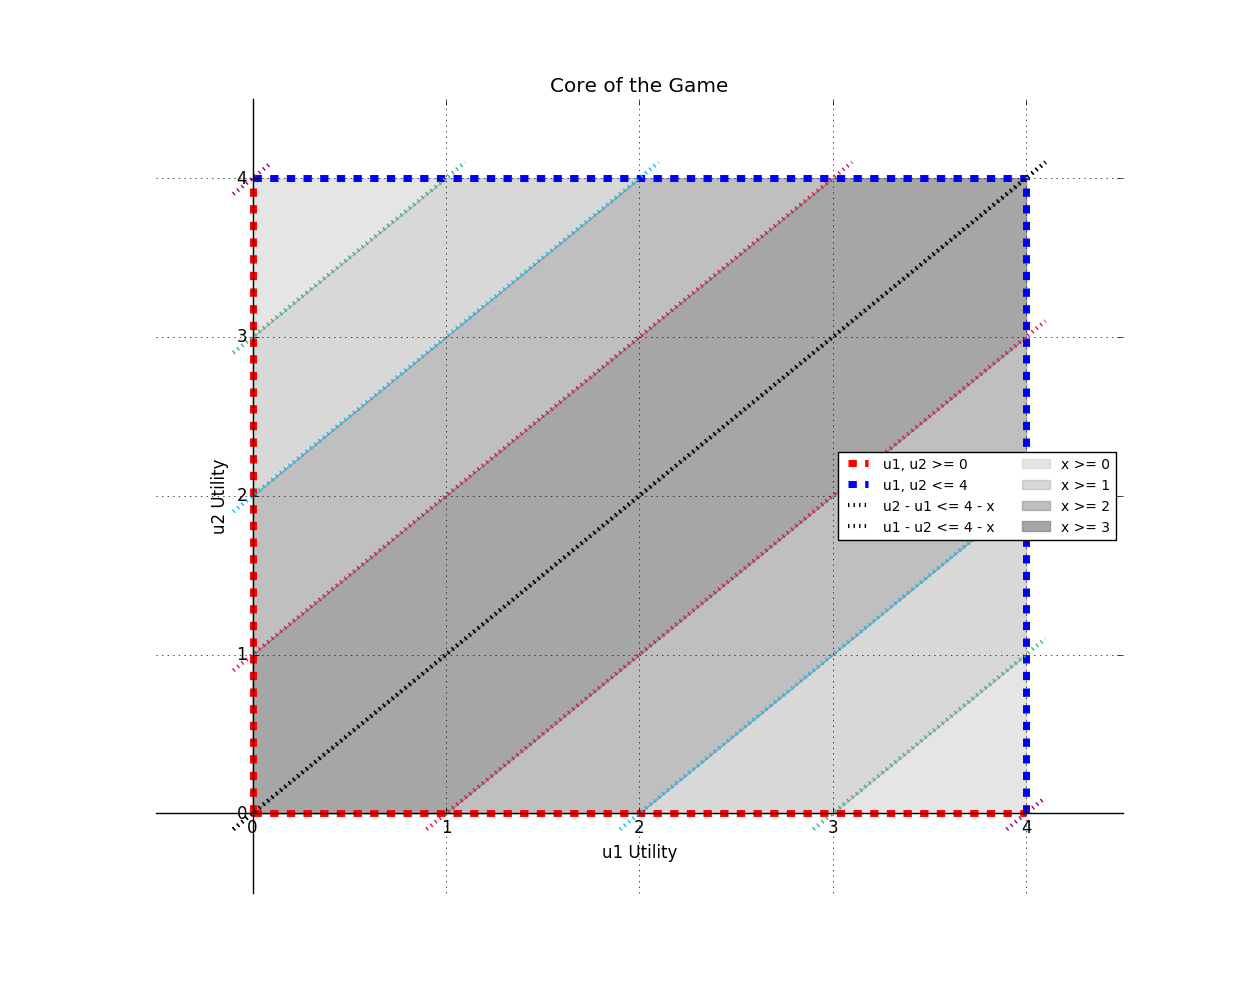
\includegraphics[width=.8\linewidth]{03-a}
      \caption{A graph of the core of the game in terms of utility payoffs for the sellers.}
      \label{fig:05_b}
    \end{figure}
    %
    % Python Plot Code
    %
    % import matplotlib.pyplot as pp
    % from matplotlib.font_manager import FontProperties
    %
    %
    % fig, ax = pp.subplots()
    %
    % fig.patch.set_facecolor('white')
    % ax.grid(True, 'both')
    % ax.spines['left'].set_position('zero')
    % ax.spines['right'].set_color('none')
    % ax.spines['bottom'].set_position('zero')
    % ax.spines['top'].set_color('none')
    %
    % pp.title('Core of the Game')
    % pp.xlabel('u1 Utility')
    % pp.ylabel('u2 Utility')
    %
    % limits = [-0.5, 4.5]
    % pp.xlim(*limits)
    % pp.ylim(*limits)
    %
    % line_opts = {'linestyle': '--', 'linewidth': 5}
    %
    % pp.plot([0, 0], [0, 4], label='u1, u2 >= 0', color='red', **line_opts)
    % pp.plot([0, 4], [0, 0], color='red', **line_opts)
    % pp.plot([4, 4], [0, 4], label='u1, u2 <= 4', color='blue', **line_opts)
    % pp.plot([0, 4], [4, 4], color='blue', **line_opts)
    %
    % line_opts = {'linestyle': ':', 'linewidth': 3}
    %
    % # x = 0
    % x = [-0.1, 0.1]
    % y = [3.9, 4.1]
    % pp.plot(x, y, color='darkmagenta', **line_opts)
    % pp.plot(y, x, color='darkmagenta', **line_opts)
    % # x = [0, 0]
    % # y = [4, 4]
    % # pp.fill_between(x, y, color=(0.5, 0.5, 0.5, 0.1))
    % # pp.fill_between(y, x, color=(0.5, 0.5, 0.5, 0.1))
    %
    % # x = 1
    % x = [-0.1, 1.1]
    % y = [2.9, 4.1]
    % pp.plot(x, y, color='mediumseagreen', **line_opts)
    % pp.plot(y, x, color='mediumseagreen', **line_opts)
    % x = [0, 1]
    % y = [3, 4]
    % y2 = [4, 4]
    % pp.fill_between(x, y, y2, color=(0.5, 0.5, 0.5, 0.2), label='x >= 0')
    % x = [3, 4]
    % y = [0, 0]
    % y2 = [0, 1]
    % pp.fill_between(x, y, y2, color=(0.5, 0.5, 0.5, 0.2))
    %
    % x = [-0.1, 2.1]
    % y = [1.9, 4.1]
    % pp.plot(x, y, color='deepskyblue', **line_opts)
    % pp.plot(y, x, color='deepskyblue', **line_opts)
    % x = [0, 1, 2]
    % y = [2, 3, 4]
    % y2 = [3, 4, 4]
    % pp.fill_between(x, y, y2, color=(0.5, 0.5, 0.5, 0.3), label='x >= 1')
    % x = [2, 3, 4]
    % y = [0, 0, 1]
    % y2 = [0, 1, 2]
    % pp.fill_between(x, y, y2, color=(0.5, 0.5, 0.5, 0.3))
    %
    %
    % x = [-0.1, 3.1]
    % y = [0.9, 4.1]
    % pp.plot(x, y, color='crimson', **line_opts)
    % pp.plot(y, x, color='crimson', **line_opts)
    % x = [0, 2, 3]
    % y = [1, 3, 4]
    % y2 = [2, 4, 4]
    % pp.fill_between(x, y, y2, color=(0.5, 0.5, 0.5, 0.5), label='x >= 2')
    % x = [1, 2, 4]
    % y = [0, 0, 2]
    % y2 = [0, 1, 3]
    % pp.fill_between(x, y, y2, color=(0.5, 0.5, 0.5, 0.5))
    %
    %
    % x = [0, 3, 4]
    % y = [0, 3, 4]
    % y2 = [1, 4, 4]
    % pp.fill_between(x, y, y2, color=(0.5, 0.5, 0.5, 0.7), label='x >= 3')
    % x = [0, 1, 4]
    % y = [0, 0, 3]
    % y2 = [0, 1, 4]
    % pp.fill_between(x, y, y2, color=(0.5, 0.5, 0.5, 0.7))
    %
    % pp.plot([-0.1, 4.1], [-0.1, 4.1],  color='black', label='u2 - u1 <= 4 - x', **line_opts)
    % pp.plot([-0.1, 4.1], [-0.1, 4.1],  color='black', label='u1 - u2 <= 4 - x', **line_opts)
    %
    %
    % font_prop = FontProperties()
    % font_prop.set_size('small')
    % pp.legend(loc='center right', ncol=2, prop=font_prop)
    % pp.show()

    We have $\mu^{*} = \{(i=1, j=1), (i=2, j=2)\}$

    For condition (1) (of the conditions for a vector to be in the core of an assignment game) we have:
    \begin{align*}
    u_{1} + v_{1} &= 4 \\
    u_{2} + v_{2} &= 4
    \end{align*}

    For condition (2) we have:
    \begin{align*}
    u_{1} + v_{2} &\ge x \\
    u_{2} + v_{1} &\ge x
    \end{align*}
    
    For condition (3) we have: $u_{1} \ge 0, u_{2} \ge 0, v_{1} \ge 0, v_{2} \ge 0$ \\

    For condition (4), there is no constraint since all of the sellers were matched. \\

    For condition (5), there is no constraint since all of the buyers were matched. \\

    Solving for the $v_{i}$ in terms of the $u_{i}$ (using the equations from condition (1)), we have:
    \begin{align*}
    v_{1} &= 4 - u_{1} \\
    v_{2} &= 4 - u_{2}
    \end{align*}

    This gives the constraints (in terms of the seller's utility):
    \begin{align*}
    u_{1} - u_{2} &\ge 4 - x \\
    u_{2} - u_{1} &\ge 4 - x \\
    u_{1}         &\ge 0     \\
    u_{2}         &\ge 0     \\
    u_{1}         &\le 4     \\
    u_{2}         &\le 4     \\
    \end{align*}

    %
    \item Find the area of the region you graphed as a function of $x$. \\

    \textit{Solution}: \\
    \[A_{core} = 16 - x^{2}\]

    The core is a $4 \times 4$ square when $x = 0$, and the $x$ constraints cut off triangular sections from the square as $x$ grows, so we have:
    \[A_{core} = 4^{2} - 2(\frac{1}{2} * x * x) \implies A_{core} = 16 - x^{2}\] 

    %
    \item We may think of $x$ as a measure of ``competition" in the market, in that $2x$ is the surplus generated by the second ``second-most-maximal" matching. State a general observation on the size of the core as a function of the amount of ``competition" in the game. \\

    \textit{Solution}: \\
    
    As the ``competition" between buyers increases, the size of the core decreases. However, seller's can still realize maximum payoff ($u_{1} = u_{2} = 4$) at any core size. \\

    %
    \end{enumerate}

\item A \textit{doubly stochastic matrix} is an $n \times n$ nonnegative matrix whose row and column sums are all $1$. A \textit{permutation matrix} is a doubly stochastic matrix in which all elements are either $0$ or $1$.

In other words, if $D$ is a doubly stochastic matrix, then there exists $K$ permutation matrices $P^{1} \dots P^{k}$, and a probability vector $(\alpha_{1}, \dots, \alpha_{k})$, with $D = \alpha_{1}P^{1} + \dots + \alpha_{k}P^{k}$.

    \begin{enumerate}
    \item Write the doubly stochastic matrix
    \[
    D = \begin{pmatrix}
    \frac{1}{4}  &  0            &  \frac{3}{4}  &  0           \\[0.3em]
    \frac{1}{2}  &  0            &  \frac{1}{4}  &  \frac{1}{4} \\[0.3em]
    \frac{1}{4}  &  \frac{1}{2}  &  0            &  \frac{1}{4} \\[0.3em]
    0            &  \frac{1}{2}  &  0            &  \frac{1}{2}
    \end{pmatrix}
    \]
    as a convex combination of permutation matrices. \\

    \textit{Solution}: \\

    \[
    D = \frac{1}{4} \begin{pmatrix}
      0 & 0 & 1 & 0 \\
      1 & 0 & 0 & 0 \\
      0 & 1 & 0 & 0 \\
      0 & 0 & 0 & 1
    \end{pmatrix} +
    \frac{1}{4} \begin{pmatrix}
      0 & 0 & 1 & 0 \\
      1 & 0 & 0 & 0 \\
      0 & 0 & 0 & 1 \\
      0 & 1 & 0 & 0
    \end{pmatrix} +
    \frac{1}{4} \begin{pmatrix}
      1 & 0 & 0 & 0 \\
      0 & 0 & 1 & 0 \\
      0 & 1 & 0 & 0 \\
      0 & 0 & 0 & 1
    \end{pmatrix} +
    \frac{1}{4} \begin{pmatrix}
      0 & 0 & 1 & 0 \\
      0 & 0 & 0 & 1 \\
      1 & 0 & 0 & 0 \\
      0 & 1 & 0 & 0
    \end{pmatrix}
    \]

    Note that permutation matrices are doubly stochastic in addition to being binary. A convex conbination is a linear combination where all coefficients are non-negative and sum to $1$. \\

    %
    \item We can use the Birkhoff-Von Neumann theorem to re-prove the result from class that the assignment of linear program ($ALP$) always solves with an integer solution, at least in the case where $l = m$. (Note that any assignment game can be made to be this way by simply adding dummy sellers whose goods have no value or dummy buyers who do not value goods to create an equivalent game where $l = m$)

        \begin{enumerate}
        \item First argue that if the $ALP$ has an optimal solution $x$, it must have another optimal solution $x^{*}$ in which all of the constraints hold with equality. \\

        \textit{Solution}: \\

        Knowing that $C$ is a nonnegative, and since none of the constraints limits any other constraint, it must be possible to take the elements of an optimal solution $x$ and increase them until the constraints of $ALP$ are met with equality, producing $x^{*}$. Since $x$ was optimal, $x^{*}$ must also be optimal. \\

        %
        \item Next argue that any such $x^{*}$ represents a doubly stochastic matrix; thus $x^{*} = \alpha_{1}P^{1} + \dots + \alpha_{k}P^{k}$. \\

        \textit{Solution}: \\

        If $x^{*}$ is a solution to $ALP$ and the constraints hold with equality, then each column and row sum is exactly $1$, by definition of the constraints. Also, because we make the assumption that the numbers of buyers and sellers are equal, we know that $x^{*}$ will be a square matrix. This is the definition of a doubly stochastic matrix; thus $x^{*}$ is doubly stochastic. \\

        %
        \item Next argue that $\sum{c_{ij}x_{ij}^{*}} \le \sum{c_{ij}P_{ij}^{k}}$, for at least one $k$. \\

        \textit{Solution}: \\
        % The inequality should be written with fully qualified sums:
        % \[\sum{\sum{c_{ij}x_{ij}^{*}}_{j}}_{i} \le \sum{c_{ij}P_{ij}^{k}}\]

        There must be at least on $P$ matrix whose $1$ elements are aligned with the largest elements of $C$ of each column (or row, for that matter). This must happen because the $P$ matrices must only have $1$ elements in positions where there are non-zero $x^{*}$ elements, and this means it is possible to have a $P$ matrix that is ``aligned" with the largest elements of $C$ that $x^{*}$ is ``aligned" with. Knowing this, we can say that one of these large $c_{ij}$s multiplied by $1$ from one of the $P^{k}$s will be must be greater than or equal to the sum of the the column of $x^{*}$ elements that are then multiplied by the corresponding column elements of $C$, all of which must be less than or equal to the largest $c_{ij}$ of the column (i.e. $1$ multiplied with a large number must be greater than or equal to the sum of fractions summing to one multiplied by numbers less than or equal to the large number). If this is true for every column, then $\sum{c_{ij}x_{ij}^{*}} \le \sum{c_{ij}P_{ij}^{k}}$ must be true. \\
        %
        % Since the $C$ elements won't change over the course of the sums, we can really discuss the comparison $\sum{x_{ij}^{*}} \le \sum{P_{ij}^{k}}$. Since elements of any $P$ are either $0$ or $1$, and the elements of $s^{*}$ are not necessarily integers, but both are doubly stochastic, it must be that the sum of all of the $x^{*}$ elements is less than or equal to the sum of any of the $P$ matrices. \\

        %
        \item Conclusion. \\

        \textit{Solution}: \\

        If an optimal solution $x^{*}$ is optimal, doubly stochastic and can be represented using only integers ($0$ or $1$), this it must be maximal. \\

        %
        \end{enumerate}
    %
    \end{enumerate}

%
\end{enumerate}
%
\end{document}
